\section{Novel methods}
\label{sec:methods}

\begin{figure*}[t]
\begin{center}
\centerline{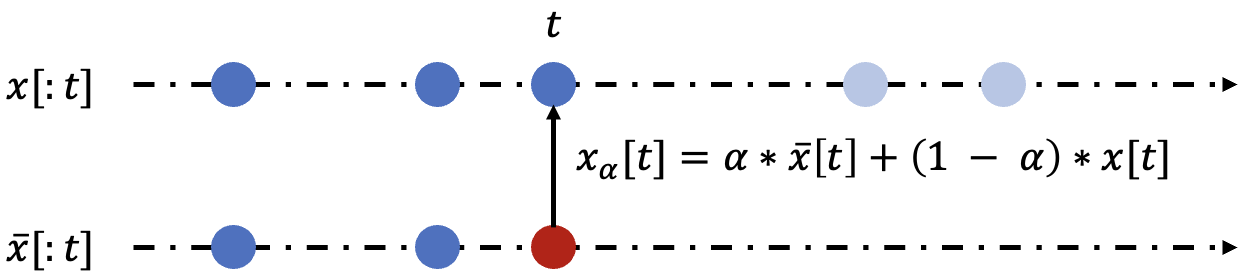
\includegraphics[width=0.6\textwidth]{figures/tig}}
\caption{
    \textbf{Illustration of the TIG method}.
    Given an input $\textbf{x}$ and a corresponding baseline $\overline{\textbf{x}}$, we compute the attribution as such.
    For each time t, we crop future times: $\textbf{x}[:t]$, and we only compute interpolations on the last data point in
    time: $\textbf{x}_{\alpha} = (x_1, x_2, \dots, \alpha \times \overline{\textbf{x}}[t] + (1 - \alpha) \times \textbf{x}[t])$.
    Using these interpolated points, we can then compute the integrated gradients.
}
\label{fig:tig}
\end{center}
\end{figure*}

We present in this section several previously unpublished methods, which have been developed
with \texttt{\detokenize{time_interpret}}.
There are two types of such methods: ones which are specific to temporal data, and others which are more general.


\subsection{Temporal attribution methods}
\label{subsec:temporal-attribution-methods}

\paragraph{Temporal Integrated Gradients.}

Temporal Integrated Gradients (TIG), illustrated on Figure~\ref{fig:tig}, adapts the original Integrated Gradients
method~\citep{sundararajan2017axiomatic} to specifically handle time-series data.
In this method, instead of directly computing attribution by summing gradients over interpolated points between the
original data $\textbf{x}$ and an uninformative baseline $\overline{\textbf{x}}$, we first crop the temporal sequence up
to a specific time t.
Then, we keep all the data points in time fixed, only computing interpolations on the last data point at time t.
The baseline of the sequence $\textbf{x} \in \mathbb{R}^{TN}$, where $T$ is the temporal dimension and $N$ the
feature dimension, can therefore be defined as:

\[ \overline{\textbf{x}}[:t] = (\textbf{x}_1, \dots, \textbf{x}_{t-1}, \overline{\textbf{x}}_t) \]

Using this baseline, we can now define TIG on time t and feature i:

\begin{equation}
    \textrm{TIG}_{ti} \coloneqq  (x_{ti} - \overline{x}_{ti}) \times
    \int_0^1 \frac{\partial \textrm{F}(\overline{\textbf{x}}[:t] + \alpha \times (\textbf{x}[:t] -
    \overline{\textbf{x}}[:t]))}{\partial x_{ti}} \, d\alpha
    \label{eq:tig}
\end{equation}

The overall attribution of a temporal point $\textbf{x}_t$ is then computed by summing over the feature dimension i and
normalising the result:

\[ \textrm{TIG}_t(\textbf{x}) \coloneqq \frac{\sum_i \textrm{TIG}_{ti}}{||\textrm{TIG}||} \]

As a result, in this setting, we keep the baseline as close as possible to the original input data, only modifying the
last input in time.
Moreover, we remove any future data points, so that they do not influence the attribution of the data point $\textbf{x}_t$.
This method can also be seen as an adaptation of SIG~\citep{enguehard2023sequential}, applied not on sequences, but on
temporal data.


\paragraph{Time Forward Tunnel.}

This method extends the one presented in~\citep{tonekaboni2020went}, allowing any Captum method to be used on temporal
data.
As such, this tool computes attribution iteratively by cropping the input data $\textbf{x} \in \mathbb{R}^{TN}$ up to
a time t, and performing the passed feature attribution method:

\[ \textrm{TimeForwardTunnel(AttrMethod)}(\textbf{x}_t) = \textrm{AttrMethod}(\textbf{x}[:t])_t \]

As a result, future data is not used when computing the attribution of a temporal data $\textbf{x}_t$.

Moreover, instead of passing a target, Time Forward Tunnel allows to use a model's predictions at time t as the target,
supporting a range of tasks: binary, multilabel, multiclass and regression ones.

Furthermore, note that TimeForwardTunnel used with IntegratedGradients is different from TIG, as the former method uses
$(\overline{\textbf{x}}_1, \dots, \overline{\textbf{x}}_t)$ as a baseline, while TIG uses
$(\textbf{x}_1, \dots, \textbf{x}_{t-1}, \overline{\textbf{x}}_t)$,
only computing interpolations on the last temporal data point.


\paragraph{Temporal attributions, targets and additional arguments.}

A number of implemented method support $``$temporal attribution$"$, meaning that, in this setting, they will return
feature attributions at each temporal point.
Therefore, if the input data is of shape $\textbf{x} \in \mathbb{R}^{TN}$, the corresponding attribution will be of
shape $\textrm{Attr} \in \mathbb{R}^{TTN}$, with an extra dimension $T$ representing the temporality of the attributions.
For instance, $\textbf{x}_t$ could be important at time $t_1$, $\textrm{Attr}_{t_1}$ having high values, but could also
be less important at a later time $t_2$, $\textrm{Attr}_{t_2}$ having lower values.

The supported methods currently are:

\begin{itemize}
    \item DynaMask
    \item ExtremalMask
    \item Fit
    \item Retain
    \item Temporal IG
    \item Time Forward Tunnel
\end{itemize}


\subsection{Other attribution methods}
\label{subsec:other-attribution-methods}

\paragraph{Local Outlier Factor (LOF) LIME and Kernel SHAP\@.}

LOF LIME and LOF Kernel SHAP are variations of the vanilla methods LIME and SHAP, using the Local Outlier Factor
score~\citep{breunig2000lof} as an indication of similarity between the masked data and the original one:

\[ \textrm{SimilarityScore}(\textbf{x}; X) = \frac{1}{\max(1, \textrm{LOF}(\textbf{x}, X))} \]

where \textbf{x} is a data point to be explained, and $X$ is a set of data points.
A low value of LOF indicates an inlier, while a large value an outlier.
As a result, SimilarityScore is lower when \textbf{x} is an outlier.

This similarity measure is then used as a weight of the interpretable sample for training an interpretable model.
Therefore, with these methods, it matters less how different a masked data point is, compared with the original one.
What matters here is how far the masked data point is from a data distribution.
These methods should therefore be less sensitive to outliers.
However, to properly work, they require a number of data points to be used as the original data distribution.


\paragraph{Non-linearities tunnel.}

This method expands the work of~\citep{dombrowski2019explanations}, by replacing some of a model's modules before
computing feature attributions.
By default, this tool replaces ReLU activations with Softplus ones, in order to reduce the potential to manipulate
explanations due to a predictive space with a high curvature, as explored by~\citep{dombrowski2019explanations}.
However, any module could similarly be replaced here.
